\documentclass{article}\usepackage[]{graphicx}\usepackage[]{color}
% maxwidth is the original width if it is less than linewidth
% otherwise use linewidth (to make sure the graphics do not exceed the margin)
\makeatletter
\def\maxwidth{ %
  \ifdim\Gin@nat@width>\linewidth
    \linewidth
  \else
    \Gin@nat@width
  \fi
}
\makeatother

\definecolor{fgcolor}{rgb}{0.345, 0.345, 0.345}
\newcommand{\hlnum}[1]{\textcolor[rgb]{0.686,0.059,0.569}{#1}}%
\newcommand{\hlstr}[1]{\textcolor[rgb]{0.192,0.494,0.8}{#1}}%
\newcommand{\hlcom}[1]{\textcolor[rgb]{0.678,0.584,0.686}{\textit{#1}}}%
\newcommand{\hlopt}[1]{\textcolor[rgb]{0,0,0}{#1}}%
\newcommand{\hlstd}[1]{\textcolor[rgb]{0.345,0.345,0.345}{#1}}%
\newcommand{\hlkwa}[1]{\textcolor[rgb]{0.161,0.373,0.58}{\textbf{#1}}}%
\newcommand{\hlkwb}[1]{\textcolor[rgb]{0.69,0.353,0.396}{#1}}%
\newcommand{\hlkwc}[1]{\textcolor[rgb]{0.333,0.667,0.333}{#1}}%
\newcommand{\hlkwd}[1]{\textcolor[rgb]{0.737,0.353,0.396}{\textbf{#1}}}%
\let\hlipl\hlkwb

\usepackage{framed}
\makeatletter
\newenvironment{kframe}{%
 \def\at@end@of@kframe{}%
 \ifinner\ifhmode%
  \def\at@end@of@kframe{\end{minipage}}%
  \begin{minipage}{\columnwidth}%
 \fi\fi%
 \def\FrameCommand##1{\hskip\@totalleftmargin \hskip-\fboxsep
 \colorbox{shadecolor}{##1}\hskip-\fboxsep
     % There is no \\@totalrightmargin, so:
     \hskip-\linewidth \hskip-\@totalleftmargin \hskip\columnwidth}%
 \MakeFramed {\advance\hsize-\width
   \@totalleftmargin\z@ \linewidth\hsize
   \@setminipage}}%
 {\par\unskip\endMakeFramed%
 \at@end@of@kframe}
\makeatother

\definecolor{shadecolor}{rgb}{.97, .97, .97}
\definecolor{messagecolor}{rgb}{0, 0, 0}
\definecolor{warningcolor}{rgb}{1, 0, 1}
\definecolor{errorcolor}{rgb}{1, 0, 0}
\newenvironment{knitrout}{}{} % an empty environment to be redefined in TeX

\usepackage{alltt}
\usepackage{Sweave}
\usepackage{float}
\usepackage{subcaption}
\usepackage{graphicx}
\usepackage{tabularx}
\usepackage{siunitx}
\usepackage{multirow}
\usepackage{amssymb} % for math symbols
\usepackage{amsmath} % for aligning equations
%\usepackage{hyperref}
\usepackage{textcomp}
\usepackage{mdframed}
\usepackage{longtable}
\usepackage{natbib}
\bibliographystyle{..//bib/styles/gcb}
%\usepackage[hyphens]{url}
\usepackage{caption}
\setlength{\captionmargin}{30pt}
\setlength{\abovecaptionskip}{0pt}
\setlength{\belowcaptionskip}{10pt}
\topmargin -1.5cm        
\oddsidemargin -0.04cm   
\evensidemargin -0.04cm
\textwidth 16.59cm
\textheight 21.94cm 
%\pagestyle{empty} %comment if want page numbers
\parskip 7.2pt
\renewcommand{\baselinestretch}{1.5}
\parindent 0pt
\usepackage{lineno}
\linenumbers

\newmdenv[
  topline=true,
  bottomline=true,
  skipabove=\topsep,
  skipbelow=\topsep
]{siderules}

%% R Script


\IfFileExists{upquote.sty}{\usepackage{upquote}}{}
\begin{document}
\noindent 
\textbf{\LARGE{Climate change reshapes the drivers of false spring risk across European trees}} 
%\\
%OR \\
%\textbf{\Large{Climate change increases the risk of false springs in European trees}} \\ % Lizzie votes for the first title! Reviewers can ask you to make it more narrow so I would start here and shift to Ben's if requested ... (goal 1: get paper out for review)
%\textbf{\Large{False spring risk increases across European trees in the face of climate change}}



\noindent Authors:\\
C. J. Chamberlain $^{1,2}$, B. I. Cook $^{3}$, I. Morales-Castilla $^{4,5}$ \& E. M. Wolkovich $^{1,2,6}$
\vspace{2ex}\\
\emph{Author affiliations:}\\
$^{1}$Arnold Arboretum of Harvard University, 1300 Centre Street, Boston, Massachusetts, USA; \\
$^{2}$Organismic \& Evolutionary Biology, Harvard University, 26 Oxford Street, Cambridge, Massachusetts, USA; \\
$^{3}$NASA Goddard Institute for Space Studies, New York, New York, USA; \\
$^{4}$GloCEE - Global Change Ecology and Evolution Group, Department of Life Sciences, Universidad de Alcal\'{a}, Alcal\'{a} de Henares, 28805, Spain \\
$^{5}$Department of Environmental Science and Policy, George Mason University, Fairfax, VA 22030; \\
$^{6}$Forest \& Conservation Sciences, Faculty of Forestry, University of British Columbia, 2424 Main Mall, Vancouver, BC V6T 1Z4\\
\vspace{2ex}
$^*$Corresponding author: 248.953.0189; cchamberlain@g.harvard.edu\\

\renewcommand{\thetable}{S\arabic{table}}
\renewcommand{\thefigure}{S\arabic{figure}}
\renewcommand{\labelitemi}{$-$}
\setkeys{Gin}{width=0.8\textwidth}

\section*{Methods: Spatial predictor} %I'm not too sure about the 'space parameter' terminology, I'd rather use either spatial or geographic predictor or proxy. I'm using spatial predictor, but all our predictors are spatial, so please feel free to change.

Spatial autocorrelation (SA) is a common issue in spatial ecology given that nearby spatial units tend to be more similar than units far apart, and thus, cannot be considered as independent units, which is a frequent assumption in statistical tests \citep{diniz2003spatial}. If model residuals are spatially autocorrelated, and thus, non-independent then model coefficients and errors may be biased in a hard-to-predict way \citep{mauricio2009coefficient}. On the contrary, if model residuals are not autocorrelated, then SA should not be of concern \citep{hawkins2012eight}.\\

To control for spatial autocorrelation and to account for spatially structured processes independent from our environmental predictors of false springs, we generated an additional spatial predictor for the model. To avoid collinearity, we computed our spatial predictor from the residuals of a linear model of false springs as a function (Equation S1) of all other factors that are also spatially structured (e.g. spring temperature, altitude, distance to the coast), following the logic of spatial filter modelling \citep{diniz2005modelling}. The calculation of the spatial predictor followed the next steps: (a) we fit a linear model of false spring versus environmental factors, (b) we extracted the residuals of the regression Equation S1, which represent the portion of the variation in the number of false springs that is independent from the predictors in the model and (c) we utilized the residuals as our \textit{y\textsubscript{i}} values in a selection of spatial eigenvectors to retain only the minimal subset of spatial eigenvectors that are able to remove SA from model residuals. Specifically, we selected eigenvectors following the the minimization of Moran's \textit{I} of the residuals (MIR) approach \citep{griffith2006spatial,diniz2012selection,Baumen2017}. (d) Next, we fit a linear model between the residuals of Equation S1 and the subset of selected eigenvectors. And, finally, (e) we took the fitted values from this regression as our spatial predictor in our final model (see equation from main text, Equation 1), which can be interpreted as a latent variable summarizing the spatial structure in false springs that is unaccounted for by the rest of the environmental factors in our model \citep{morales2012imprint}. A spatial predictor generated in this way has three major advantages. First, it ensures that no SA is left in model residuals. Second, it avoids introducing collinearity issues with other predictors in the model. And third, it can be interpreted as a latent variable summarizing spatial processes (e.g. local adaptation, plasticity, etc.) occurring at multiple scales.

\begin{align*}
y_i = \alpha_{[i]} +&  \beta_{NAO_{[i]}} + \beta_{MST_{[i]}} + \beta_{Elevation_{[i]}} + \beta_{DistanceCoast_{[i]}} \\ +& \beta_{ClimateChange_{[i]}}
+ \beta_{NAO \times Species_{[i]}} + \beta_{MST \times Species_{[i]}} + \beta_{Elevation \times Species_{[i]}} \\ +& \beta_{DistanceCoast \times Species_{[i]}} + \beta_{ClimateChange \times Species_{[i]}} \\
+& \beta_{NAO \times ClimateChange_{[i]}} + \beta_{MST \times ClimateChange_{[i]}} 
+ \beta_{Elevation \times ClimateChange_{[i]}} \\ +& \beta_{DistanceCoast \times ClimateChange_{[i]}} + \sigma_{[i]} \tag{S1}
\end{align*}


\section*{Species rate of budburst calculations}
Due to the paucity of data for BBCH 7 in the PEP725 dataset, we were unable to use observations for both budburst and leafout to determine the durations of vegetative risk. Instead, we used data from a growth chamber experiment \citep{Flynn2018} to determine the average number of days between budburst and leafout for our study species. We took the mean number of days between budburst and leafout for the entire experiment, which was 12 days. We compared this number to a field observation study \citep{Donnelly2017} that looked at the time between budburst and leafout across 10 species over 5 years. Finally, we assessed data that were provided by the USA National Phenology Network and the many participants who contribute to its Nature's Notebook program (USA-NPN,2019; www.usanpn.org/data/observational) for \textit{Aesculus flava} (Sol.), \textit{Aesculus glabra} (Willd.), \textit{Alnus incana} (Moench.), \textit{Betula nigra} (L.), \textit{Betula papyrifera} (Marshall), \textit{Fagus grandifolia} (Ehrh.), \textit{Fraxinus americana} (L.), \textit{Fraxinus nigra} (Marshall) and \textit{Quercus velutina} (Lam.) and took the mean number of days between budburst and leafout. Across all three approaches, the average number of days between budburst and leafout was approximately 12 days.  

Again, due to a lack of BBCH 7 data, we were unable to determine species-specific averages of number of days between budburst and leafout. We used a similar approach as above by using data from the growth chamber experiment \citep{Flynn2018} but instead of finding whole experiment means we determined species-specific averages. We used the rate of budburst of \textit{Acer saccharum} (Marshall) for \textit{Aesculus hippocastanum} \citep{Buerki2010}, \textit{Alnus incana} for \textit{Alnus glutinosa}, \textit{Betula papyrifera} for \textit{Betula pendula} \citep{Wang2016}, \textit{Fagus grandifolia} for \textit{Fagus sylvatica}, \textit{Fraxinus nigra} for \textit{Fraxinus excelsior} and \textit{Quercus alba} (L.) for \textit{Quercus robur} \citep{Hipp2017}.

\section*{Results: The effects of climatic and spatial variation on false spring incidence}
Most species had mean spring temperatures that ranged from -5$^{\circ}$C to 12$^{\circ}$C, but for \textit{Alnus glutinosa} and \textit{Fraxinus excelsior} temperatures rarely dropped below 0$^{\circ}$C, whereas \textit{Quercus robur} experienced some of the lowest spring temperatures (see Figure \ref{fig:mst}). 

The overall model output estimates are for \textit{Aesculus hippocastanum} as species were used as two-way interactions to simulate modeled groups on the main effects. For the model estimate of change plots (Figure 3, Figure \ref{fig:dvr} and Figure \ref{fig:five}), we used average predictive comparisons to calculate the mean estimates and the posteriors for each species and then took the average to find the overall effect for each predictor. The model estimates on the logit scale were converted to probability percentages for easier interpretation by using the `divide by 4' rule \citep{Gelman2006} and then back converted to the original scale. %To convert we used the equations below \citep{Gelman2006}:

\iffalse
\begin{align*}
inverselogit = & (1/(1+exp(-(Model Estimate)))) \tag{S2} 
\end{align*}
\begin{align*}
inverselogit(Intercept &+ (Model Estimate/(sd(Raw Data Predictor)*2))*mean(Raw Data Predictor)) - \\ & inverselogit(Intercept + (Model Estimate/(sd(Raw Data Predictor)*2)) \\ & *(mean(Raw Data Predictor)-(2*sd(Raw Data Predictor))) * 100 \tag{S3} 
\end{align*}
\fi

\newpage
\nocite{NPN2019}
\bibliography{..//bib/regionalrisk.bib}

\newpage
\section*{Supplement: Tables and Figures}
  
\begin{center}
\captionof{table}{Data collected from PEP725 for each species and the calculated number of false spring years} \label{tab:spp} 
\begin{tabular}{l r r r r}
\hline
Species & Num. of Observations & Num. of False Springs & Num. of Sites & Num. of Years \\
\hline
\textit{Aesculus hippocastanum} & 156468 & 44746 & 10157 & 66  \\
\textit{Alnus glutinosa} & 91094 & 27296 & 6775 & 65 \\
\textit{Betula pendula} & 154897 & 46685 & 10139 & 66 \\
\textit{Fagus sylvatica} & 129133 & 29237 & 9099 & 66 \\
\textit{Fraxinus excelsior} & 92665 & 8256 & 7327 & 65 \\
\textit{Quercus robur} & 131635 & 16657 & 8811 & 66 \\
\hline
\end{tabular}
\end{center}

\vspace{15ex}




\begin{center}
\captionof{table}{Mean day of budburst and standard deviation for each species for before (1951-1983) and after climate change (1984-2016).}
\begin{tabular}{l c c| c c}
\cline{2-5}
& \multicolumn{2}{ c| }{1951-1983}
& \multicolumn{2}{ c }{1984-2016} \\ \cline{2-5}
& mean & sd & mean & sd \\
\hline
\textit{Aesculus hippocastanum} & 102.2 & 12.44 & 95.35 & 12.09  \\
\textit{Alnus glutinosa} & 102.8 & 14.81 & 94.90 & 14.71 \\
\textit{Betula pendula} & 101.3 & 11.76 & 95.44 & 11.25 \\
\textit{Fagus sylvatica} & 109.1 & 9.978 & 103.7 & 9.623 \\
\textit{Fraxinus excelsior} & 119.4 & 11.79 & 113.5 & 11.53 \\
\textit{Quercus robur} & 115.9 & 11.31 & 109.6 & 10.95 \\
\hline
\end{tabular}
\end{center}

{\begin{figure} [H]
  -\begin{center}
  -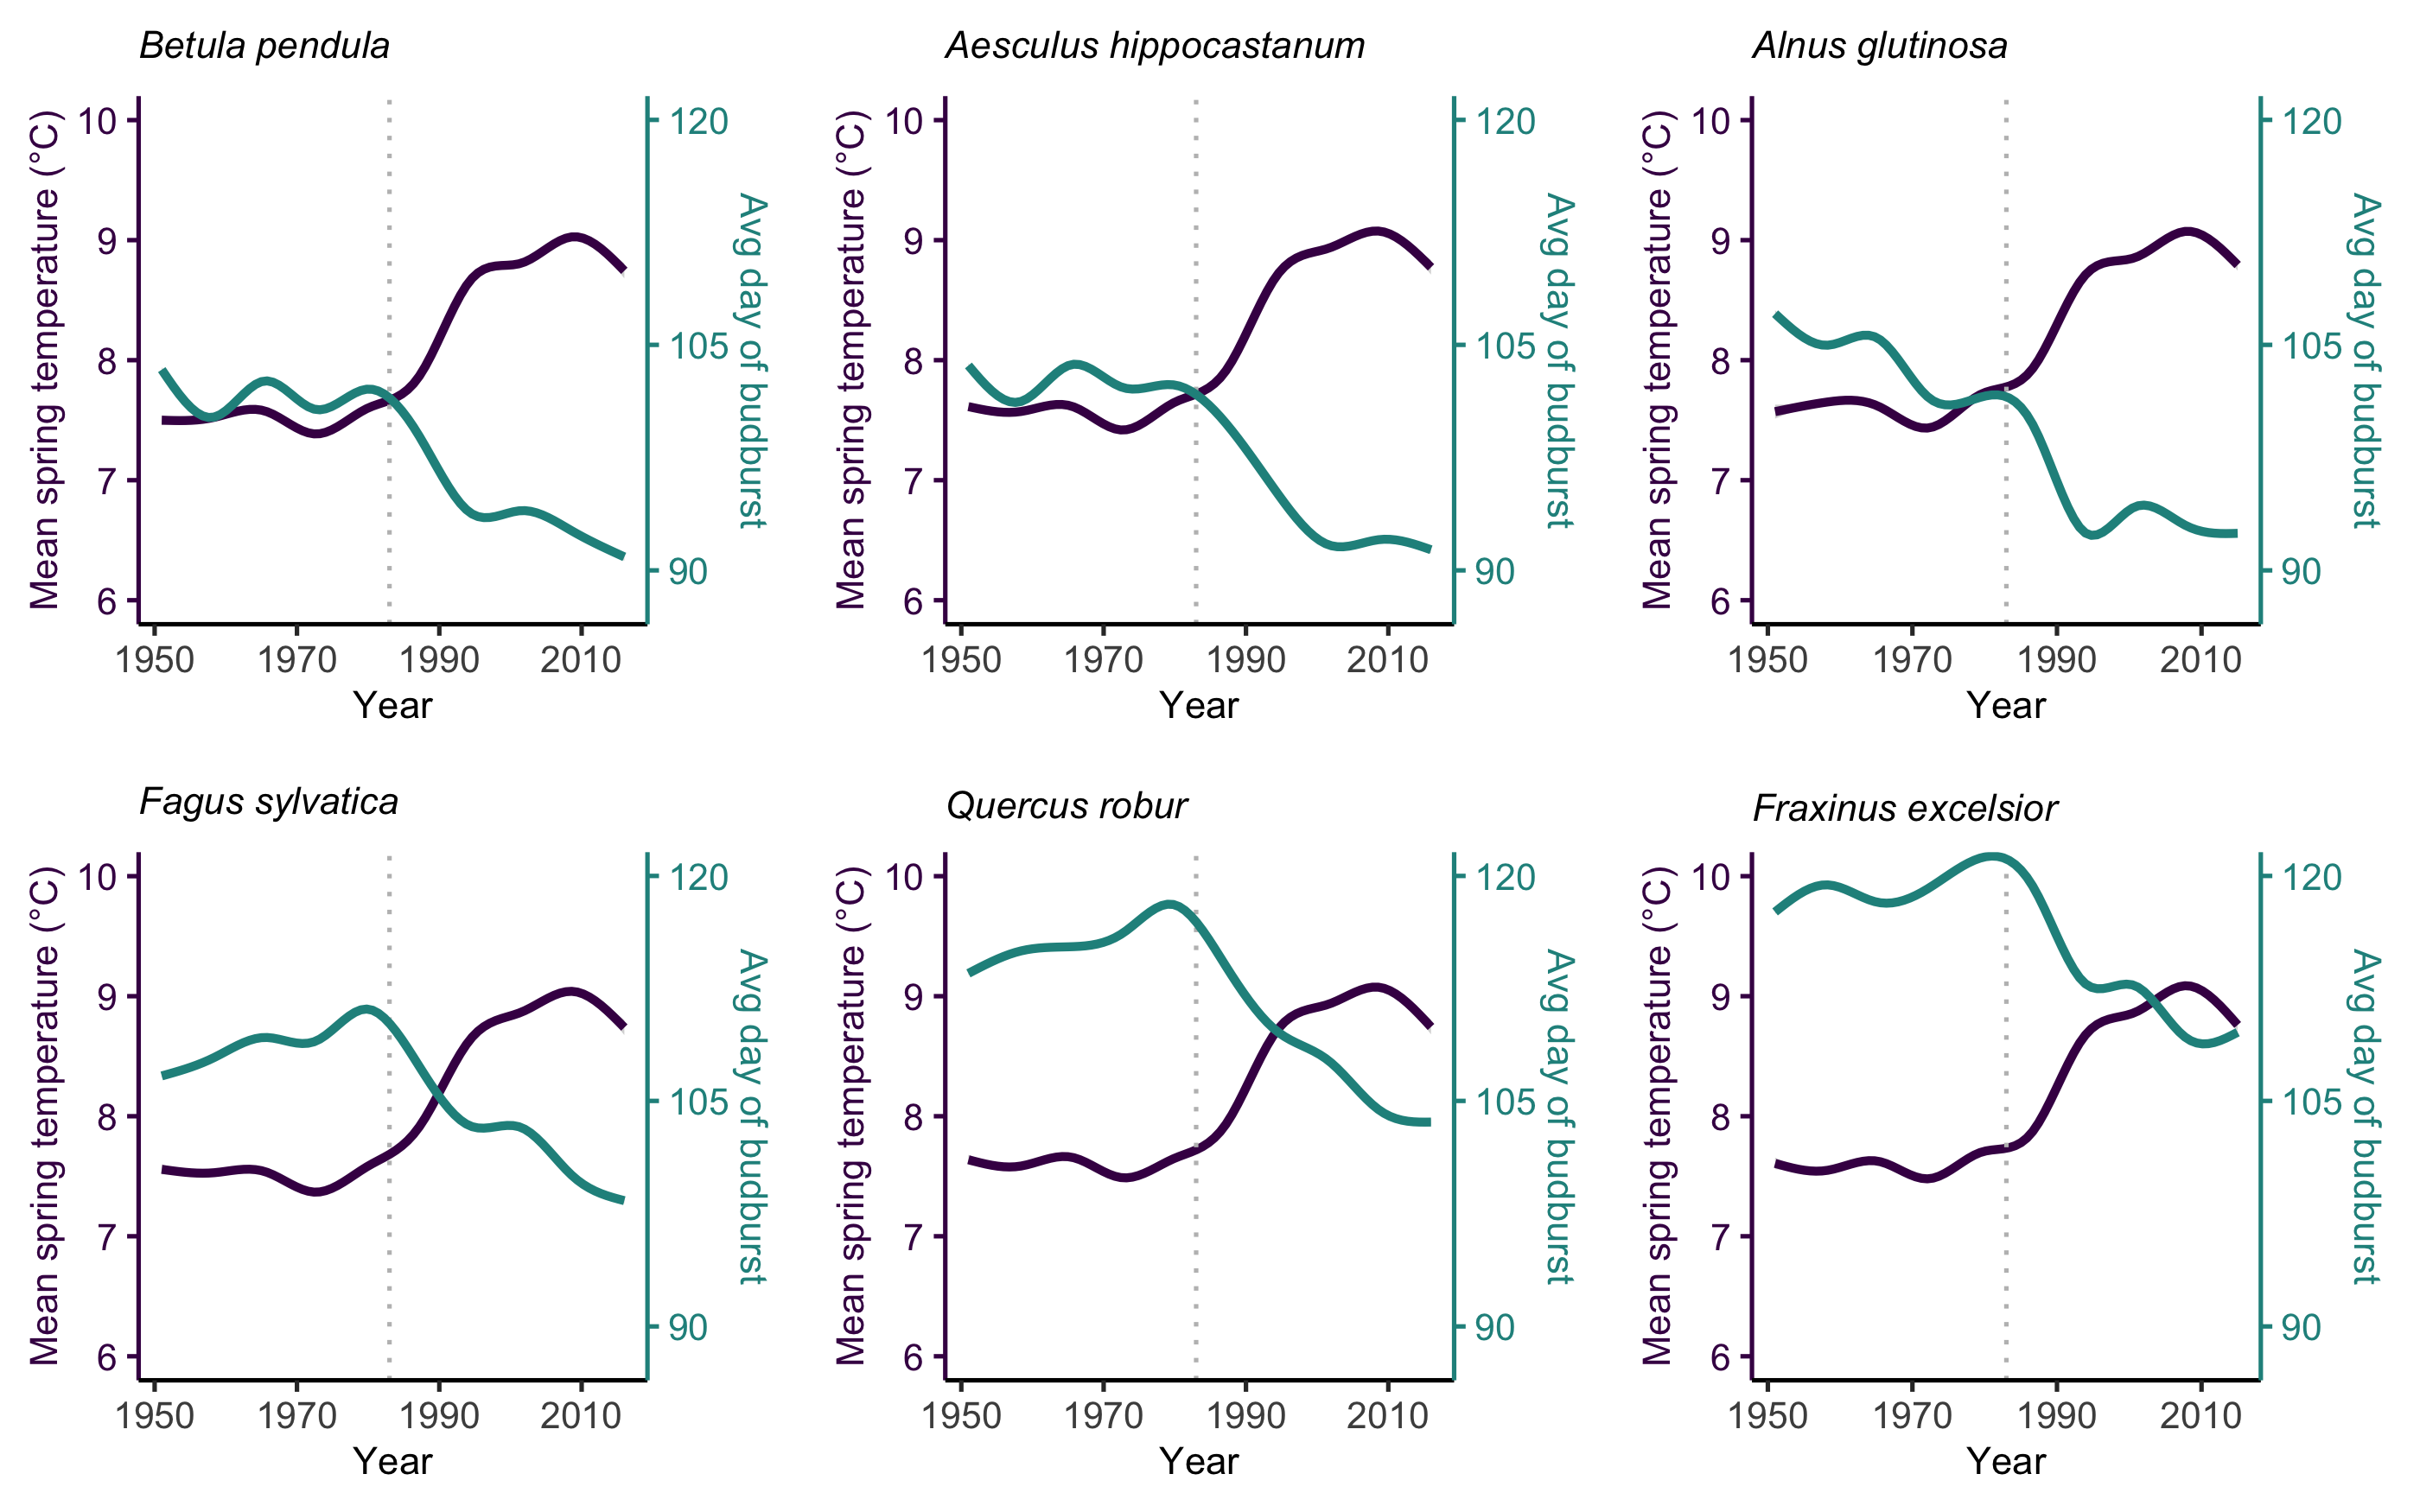
\includegraphics[width=16cm]{..//analyses/figures/MSTBB_bySpp_lines.png}
  -\caption{Mean spring temperatures are plotted for each site and year (from 1951-2016) for each species. The purple line shows the trend in mean spring temperatures from March 1 to May 31 and the green line represents the trend of average day of budburst for each year for each species. Both lines are cyclic penalized cubic regression spline smooths with basis dimensions equal to the number of years in the study (i.e., 66). Species are ordered by average day of budburst, with the earliest being \textit{Betula pendula} and the latest being \textit{Fraxinus excelsior}. }\label{fig:mst}
  -\end{center}
  -\end{figure}}


% latex table generated in R 3.6.0 by xtable 1.8-4 package
% Fri Oct  4 09:51:51 2019
\begin{table}[H]
\centering
\caption{Summary of simple linear regression model of day of budburst before and after climate change across species.} 
\begin{tabular}{lrrr}
  \hline
 & Estimate & 10\% & 90\% \\ 
  \hline
Intercept & 102.27 & 102.20 & 102.33 \\ 
  Climate Change & -6.98 & -7.08 & -6.89 \\ 
  Alnus glutinosa & 0.61 & 0.50 & 0.72 \\ 
  Betula pendula & -0.89 & -0.98 & -0.80 \\ 
  Fagus sylvatica & 6.85 & 6.75 & 6.94 \\ 
  Fraxinus excelsior & 17.16 & 17.05 & 17.28 \\ 
  Quercus robur & 13.67 & 13.57 & 13.77 \\ 
  Climate Change by Alnus glutinosa & -0.97 & -1.13 & -0.81 \\ 
  Climate Change by Betula pendula & 1.06 & 0.92 & 1.21 \\ 
  Climate Change by Fagus sylvatica & 1.61 & 1.47 & 1.76 \\ 
  Climate Change by Fraxinus excelsior & 1.07 & 0.91 & 1.24 \\ 
  Climate Change by Quercus robur & 0.67 & 0.52 & 0.81 \\ 
   \hline
\end{tabular}
\end{table}
% latex table generated in R 3.6.0 by xtable 1.8-4 package
% Fri Oct  4 09:51:53 2019
\begin{table}[H]
\centering
\caption{Summary of simple linear regression model of average minimum temperature between budburst and leafout before and after climate change across species.} 
\begin{tabular}{lrrr}
  \hline
 & Estimate & 10\% & 90\% \\ 
  \hline
Intercept & 5.99 & 5.97 & 6.00 \\ 
  Climate Change & 0.83 & 0.81 & 0.85 \\ 
  Alnus glutinosa & 1.65 & 1.63 & 1.67 \\ 
  Betula pendula & 0.50 & 0.48 & 0.52 \\ 
  Fagus sylvatica & 1.50 & 1.48 & 1.51 \\ 
  Fraxinus excelsior & 2.76 & 2.74 & 2.78 \\ 
  Quercus robur & 1.88 & 1.87 & 1.90 \\ 
  Climate Change by Alnus glutinosa & -0.04 & -0.07 & -0.01 \\ 
  Climate Change by Betula pendula & -0.31 & -0.34 & -0.29 \\ 
  Climate Change by Fagus sylvatica & 0.08 & 0.05 & 0.10 \\ 
  Climate Change by Fraxinus excelsior & -0.26 & -0.29 & -0.23 \\ 
  Climate Change by Quercus robur & -0.10 & -0.13 & -0.07 \\ 
   \hline
\end{tabular}
\end{table}
% latex table generated in R 3.6.0 by xtable 1.8-4 package
% Fri Oct  4 09:51:53 2019
\begin{table}[H]
\centering
\caption{Summary of simple linear regression model of probability of false spring before and after climate change across species.} 
\begin{tabular}{lrrr}
  \hline
 & Estimate & 10\% & 90\% \\ 
  \hline
Intercept & 0.27 & 0.27 & 0.27 \\ 
  Climate Change & 0.04 & 0.03 & 0.04 \\ 
  Alnus glutinosa & 0.00 & -0.00 & 0.00 \\ 
  Betula pendula & 0.01 & 0.01 & 0.02 \\ 
  Fagus sylvatica & -0.03 & -0.04 & -0.03 \\ 
  Fraxinus excelsior & -0.17 & -0.17 & -0.17 \\ 
  Quercus robur & -0.14 & -0.14 & -0.13 \\ 
  Climate Change by Alnus glutinosa & 0.02 & 0.02 & 0.03 \\ 
  Climate Change by Betula pendula & 0.00 & -0.00 & 0.01 \\ 
  Climate Change by Fagus sylvatica & -0.06 & -0.06 & -0.05 \\ 
  Climate Change by Fraxinus excelsior & -0.06 & -0.06 & -0.05 \\ 
  Climate Change by Quercus robur & -0.05 & -0.06 & -0.05 \\ 
   \hline
\end{tabular}
\end{table}


% latex table generated in R 3.6.0 by xtable 1.8-4 package
% Fri Oct  4 09:51:53 2019
\begin{longtable}{lrrrrr}
\caption{Summary of Bernouilli model of false spring risk with varying rates of budburst for each species without the species interactions (estimates presented on logit scale for \textit{Aesculus hippocastanum} as the intercept).} \\ 
  \hline
 & Estimate & 10\% & 25\% & 75\% & 90\% \\ 
  \hline \endhead  \hline
Intercept & -0.88 & -0.89 & -0.89 & -0.88 & -0.88 \\ 
  NAO Index & 0.14 & 0.12 & 0.13 & 0.15 & 0.16 \\ 
  Mean Spring 
Temperature & -0.48 & -0.50 & -0.49 & -0.47 & -0.45 \\ 
  Distance from 
Coast & 0.40 & 0.38 & 0.39 & 0.41 & 0.43 \\ 
  Elevation & 0.19 & 0.16 & 0.18 & 0.20 & 0.22 \\ 
  Space Parameter & -0.06 & -0.08 & -0.07 & -0.06 & -0.05 \\ 
  Climate Change & 0.35 & 0.33 & 0.34 & 0.36 & 0.37 \\ 
  Alnus glutinosa & 0.05 & 0.04 & 0.05 & 0.06 & 0.07 \\ 
  Betula pendula & 0.06 & 0.04 & 0.05 & 0.06 & 0.07 \\ 
  Fagus sylvatica & -0.35 & -0.37 & -0.36 & -0.35 & -0.34 \\ 
  Fraxinus excelsior & -1.43 & -1.45 & -1.44 & -1.42 & -1.41 \\ 
  Quercus robur & -1.03 & -1.04 & -1.03 & -1.02 & -1.01 \\ 
  NAO Index
by Alnus glutinosa & -0.07 & -0.11 & -0.09 & -0.06 & -0.04 \\ 
  NAO Index
by Betula pendula & -0.08 & -0.11 & -0.10 & -0.07 & -0.05 \\ 
  NAO Index
by Fagus sylvatica & 0.12 & 0.09 & 0.11 & 0.13 & 0.15 \\ 
  NAO Index
by Fraxinus excelsior & 0.03 & -0.02 & 0.01 & 0.05 & 0.08 \\ 
  NAO Index
by Quercus robur & 0.08 & 0.04 & 0.06 & 0.09 & 0.12 \\ 
  Mean Spring 
Temperature
by Alnus glutinosa & 0.14 & 0.10 & 0.13 & 0.16 & 0.18 \\ 
  Mean Spring 
Temperature
by Betula pendula & -0.02 & -0.05 & -0.03 & -0.01 & 0.01 \\ 
  Mean Spring 
Temperature
by Fagus sylvatica & -0.06 & -0.10 & -0.08 & -0.05 & -0.02 \\ 
  Mean Spring 
Temperature
by Fraxinus excelsior & 0.32 & 0.26 & 0.30 & 0.34 & 0.38 \\ 
  Mean Spring 
Temperature
by Quercus robur & 0.10 & 0.06 & 0.09 & 0.12 & 0.15 \\ 
  Distance from 
Coast
by Alnus glutinosa & -0.07 & -0.11 & -0.08 & -0.05 & -0.03 \\ 
  Distance from 
Coast
by Betula pendula & 0.01 & -0.02 & -0.00 & 0.03 & 0.05 \\ 
  Distance from 
Coast
by Fagus sylvatica & -0.00 & -0.04 & -0.02 & 0.01 & 0.04 \\ 
  Distance from 
Coast
by Fraxinus excelsior & 0.26 & 0.20 & 0.23 & 0.28 & 0.31 \\ 
  Distance from 
Coast
by Quercus robur & -0.10 & -0.14 & -0.12 & -0.08 & -0.05 \\ 
  Elevation
by Alnus glutinosa & 0.02 & -0.02 & 0.00 & 0.04 & 0.07 \\ 
  Elevation
by Betula pendula & 0.03 & -0.01 & 0.02 & 0.05 & 0.07 \\ 
  Elevation
by Fagus sylvatica & 0.00 & -0.04 & -0.02 & 0.02 & 0.04 \\ 
  Elevation
by Fraxinus excelsior & -0.37 & -0.43 & -0.39 & -0.34 & -0.31 \\ 
  Elevation
by Quercus robur & -0.08 & -0.13 & -0.10 & -0.06 & -0.03 \\ 
  Space Parameter
by Alnus glutinosa & 0.01 & -0.02 & 0.00 & 0.03 & 0.05 \\ 
  Space Parameter
by Betula pendula & -0.01 & -0.03 & -0.02 & 0.00 & 0.02 \\ 
  Space Parameter
by Fagus sylvatica & -0.04 & -0.07 & -0.05 & -0.03 & -0.01 \\ 
  Space Parameter
by Fraxinus excelsior & 0.05 & 0.01 & 0.03 & 0.07 & 0.09 \\ 
  Space Parameter
by Quercus robur & 0.02 & -0.02 & 0.00 & 0.03 & 0.05 \\ 
  Climate Change
by Alnus glutinosa & 0.06 & 0.03 & 0.05 & 0.07 & 0.09 \\ 
  Climate Change
by Betula pendula & 0.06 & 0.03 & 0.04 & 0.07 & 0.09 \\ 
  Climate Change
by Fagus sylvatica & -0.32 & -0.35 & -0.34 & -0.31 & -0.29 \\ 
  Climate Change
by Fraxinus excelsior & -0.52 & -0.57 & -0.54 & -0.50 & -0.47 \\ 
  Climate Change
by Quercus robur & -0.41 & -0.44 & -0.42 & -0.39 & -0.37 \\ 
  NAO Index by Climate Change & -0.83 & -0.85 & -0.84 & -0.82 & -0.81 \\ 
  Mean Spring 
Temperature by Climate Change & 0.42 & 0.40 & 0.41 & 0.43 & 0.44 \\ 
  Distance from 
Coast by Climate Change & -0.12 & -0.15 & -0.13 & -0.11 & -0.10 \\ 
  Elevation by Climate Change & -0.00 & -0.03 & -0.01 & 0.01 & 0.03 \\ 
  Space Parameter by Climate Change & -0.05 & -0.07 & -0.05 & -0.04 & -0.03 \\ 
   \hline
\hline
\end{longtable}



{\begin{figure} [H]
  -\begin{center}
  -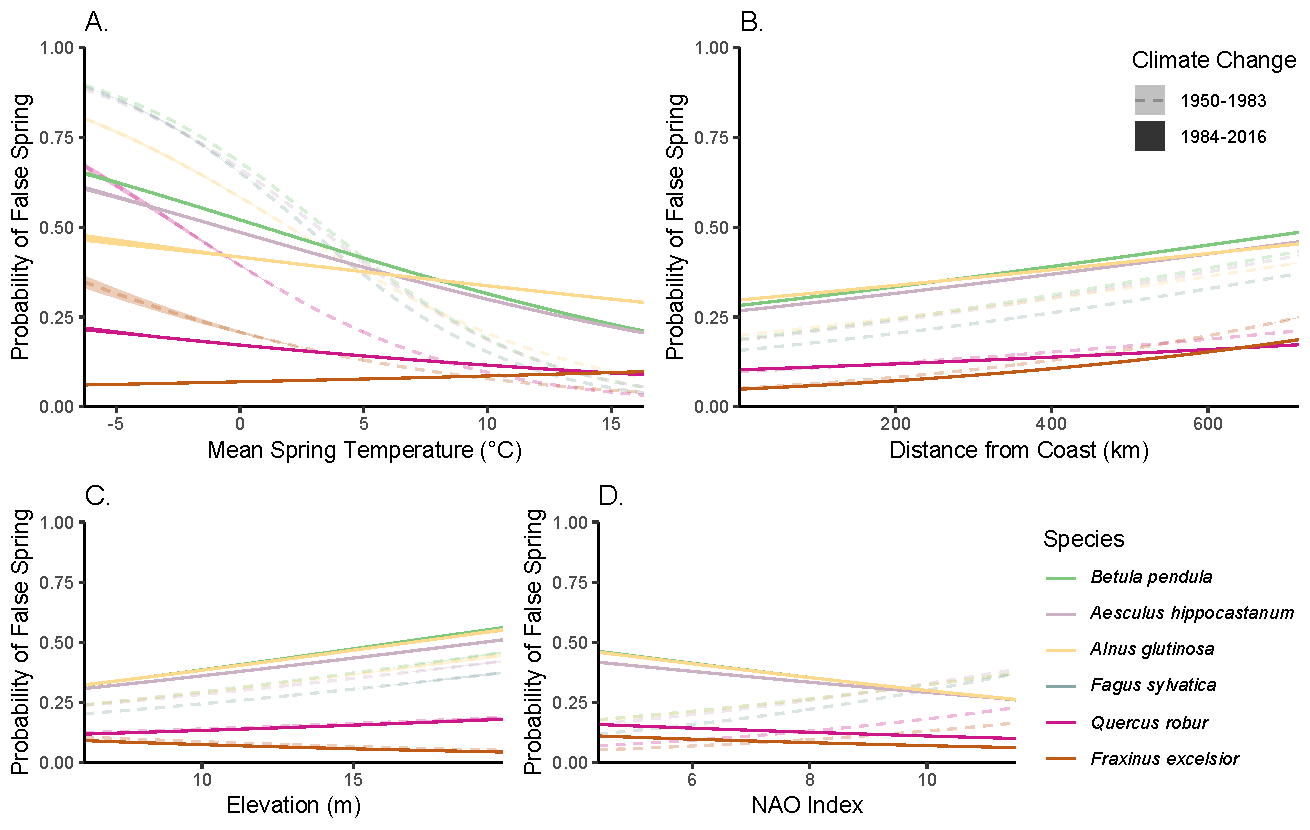
\includegraphics[width=16cm]{..//analyses/figures/APC_allpred_allspp_baseR.pdf}
  -\caption{Average predictive comparisons for all climate change interactions with each of the main effects (i.e., mean spring temperature, distance from the coast, elevation, and NAO index) for all species. }\label{fig:suppapc}
  -\end{center}
  -\end{figure}}
  
  {\begin{figure} [H]
  -\begin{center}
  -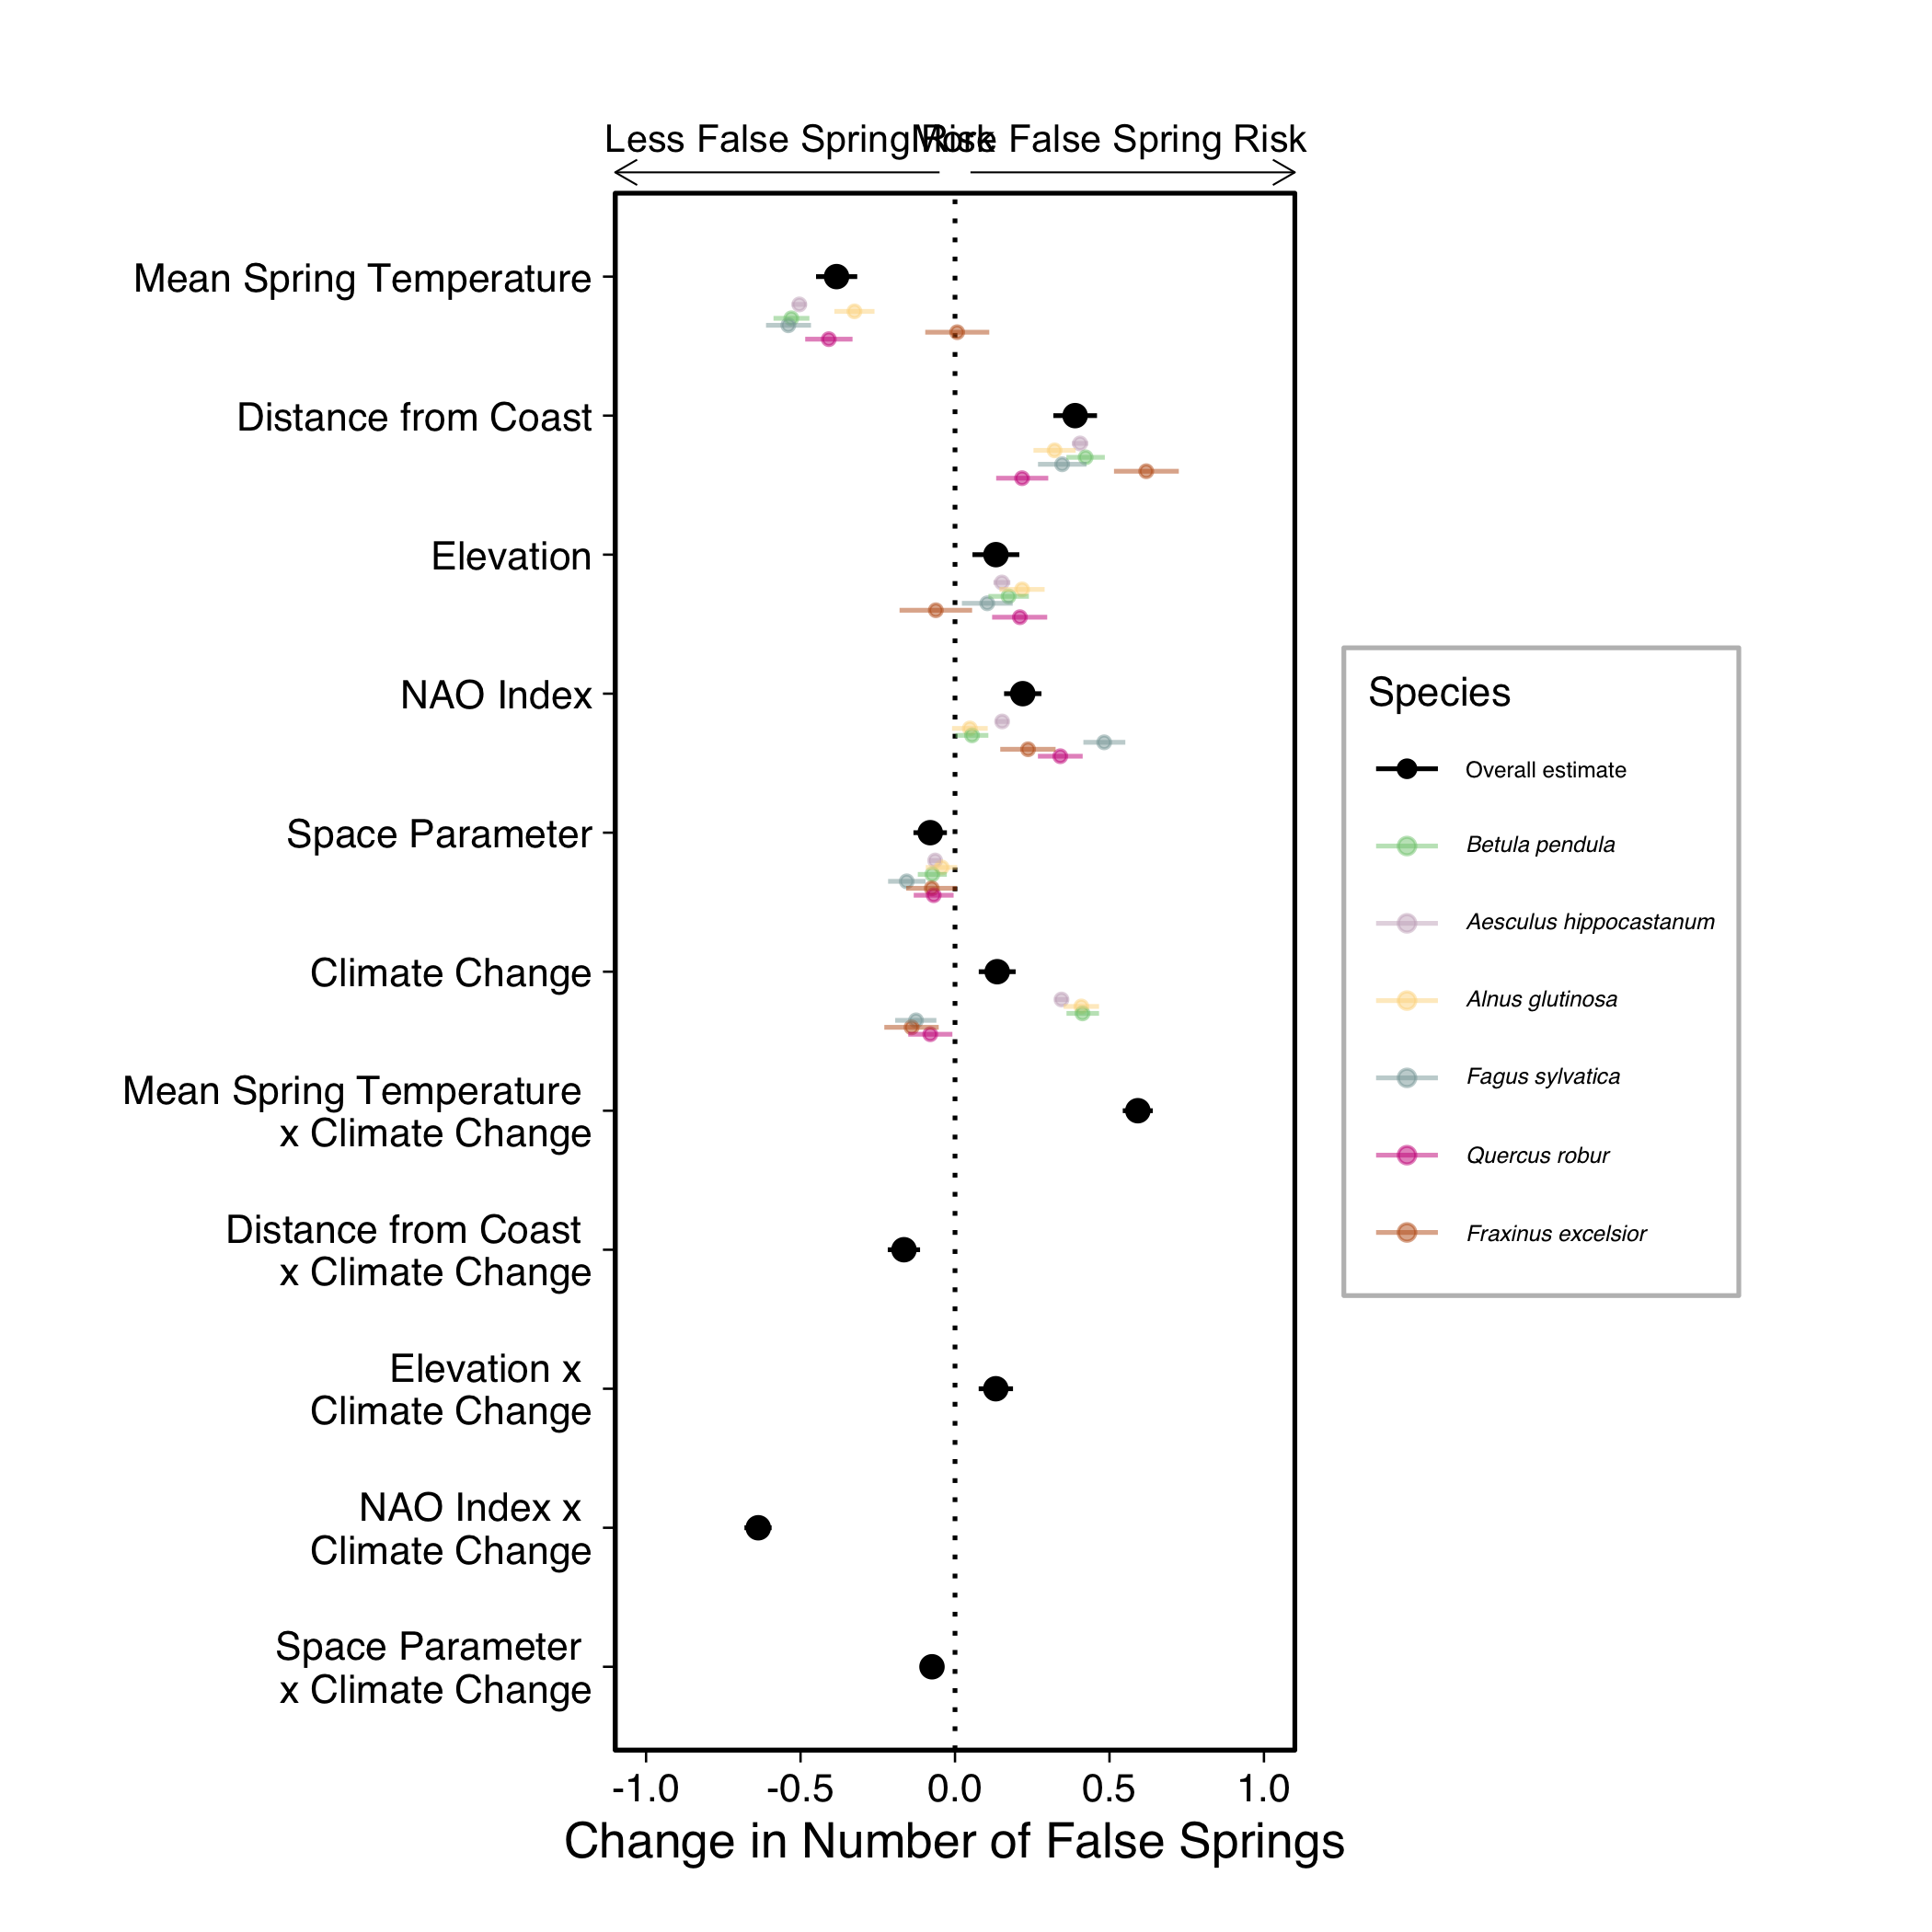
\includegraphics[width=12cm]{..//analyses/figures/model_output_90_dvrspp.png}
  -\caption{Effects of species, climatic and geographical predictors on false spring risk with different rates of leafout for each species. More positive values indicate an increased probability of a false spring whereas more negative values suggest a lower probability of a false spring. Dots and lines show means and 90\% uncertainty intervals. Values closer to zero have less of an effect on false springs. There were 622,565 zeros and 132,463 ones for false springs in the data.}\label{fig:dvr}
  -\end{center}
  -\end{figure}}
  
% latex table generated in R 3.6.0 by xtable 1.8-4 package
% Fri Oct  4 09:51:54 2019
\begin{longtable}{lrrrrr}
\caption{Summary of Bernouilli model of false spring risk with varying rates of leafout for each species without the species interactions (estimates presented on logit scale for \textit{Aesculus hippocastanum}.} \\ 
  \hline
 & Estimate & 10\% & 25\% & 75\% & 90\% \\ 
  \hline \endhead  \hline
Intercept & -1.04 & -1.05 & -1.04 & -1.03 & -1.03 \\ 
  NAO Index & 0.15 & 0.13 & 0.14 & 0.16 & 0.17 \\ 
  Mean Spring 
Temperature & -0.50 & -0.53 & -0.51 & -0.49 & -0.48 \\ 
  Distance from 
Coast & 0.40 & 0.38 & 0.39 & 0.42 & 0.43 \\ 
  Elevation & 0.15 & 0.12 & 0.14 & 0.16 & 0.18 \\ 
  Space Parameter & -0.06 & -0.08 & -0.07 & -0.06 & -0.04 \\ 
  Climate Change & 0.34 & 0.32 & 0.34 & 0.35 & 0.37 \\ 
  Alnus glutinosa & 0.20 & 0.18 & 0.19 & 0.21 & 0.22 \\ 
  Betula pendula & 0.04 & 0.03 & 0.04 & 0.05 & 0.06 \\ 
  Fagus sylvatica & -1.38 & -1.40 & -1.39 & -1.37 & -1.36 \\ 
  Fraxinus excelsior & -2.11 & -2.14 & -2.12 & -2.10 & -2.08 \\ 
  Quercus robur & -1.75 & -1.78 & -1.76 & -1.74 & -1.73 \\ 
  NAO Index
by Alnus glutinosa & -0.10 & -0.14 & -0.12 & -0.09 & -0.07 \\ 
  NAO Index
by Betula pendula & -0.10 & -0.13 & -0.11 & -0.08 & -0.07 \\ 
  NAO Index
by Fagus sylvatica & 0.33 & 0.28 & 0.31 & 0.35 & 0.38 \\ 
  NAO Index
by Fraxinus excelsior & 0.08 & 0.02 & 0.06 & 0.11 & 0.15 \\ 
  NAO Index
by Quercus robur & 0.19 & 0.14 & 0.17 & 0.21 & 0.24 \\ 
  Mean Spring 
Temperature
by Alnus glutinosa & 0.18 & 0.14 & 0.16 & 0.19 & 0.22 \\ 
  Mean Spring 
Temperature
by Betula pendula & -0.03 & -0.06 & -0.04 & -0.01 & 0.01 \\ 
  Mean Spring 
Temperature
by Fagus sylvatica & -0.04 & -0.08 & -0.06 & -0.02 & 0.01 \\ 
  Mean Spring 
Temperature
by Fraxinus excelsior & 0.51 & 0.43 & 0.48 & 0.54 & 0.59 \\ 
  Mean Spring 
Temperature
by Quercus robur & 0.10 & 0.04 & 0.07 & 0.12 & 0.15 \\ 
  Distance from 
Coast
by Alnus glutinosa & -0.08 & -0.12 & -0.10 & -0.07 & -0.04 \\ 
  Distance from 
Coast
by Betula pendula & 0.02 & -0.02 & 0.00 & 0.03 & 0.05 \\ 
  Distance from 
Coast
by Fagus sylvatica & -0.06 & -0.11 & -0.08 & -0.04 & -0.01 \\ 
  Distance from 
Coast
by Fraxinus excelsior & 0.21 & 0.14 & 0.18 & 0.25 & 0.29 \\ 
  Distance from 
Coast
by Quercus robur & -0.19 & -0.25 & -0.21 & -0.16 & -0.13 \\ 
  Elevation
by Alnus glutinosa & 0.07 & 0.02 & 0.05 & 0.08 & 0.11 \\ 
  Elevation
by Betula pendula & 0.02 & -0.02 & 0.01 & 0.04 & 0.06 \\ 
  Elevation
by Fagus sylvatica & -0.05 & -0.10 & -0.07 & -0.03 & 0.01 \\ 
  Elevation
by Fraxinus excelsior & -0.21 & -0.30 & -0.25 & -0.18 & -0.12 \\ 
  Elevation
by Quercus robur & 0.06 & -0.00 & 0.03 & 0.08 & 0.12 \\ 
  Space Parameter
by Alnus glutinosa & 0.02 & -0.01 & 0.01 & 0.03 & 0.05 \\ 
  Space Parameter
by Betula pendula & -0.01 & -0.04 & -0.02 & 0.00 & 0.02 \\ 
  Space Parameter
by Fagus sylvatica & -0.09 & -0.13 & -0.11 & -0.08 & -0.05 \\ 
  Space Parameter
by Fraxinus excelsior & -0.01 & -0.07 & -0.04 & 0.01 & 0.05 \\ 
  Space Parameter
by Quercus robur & -0.00 & -0.05 & -0.02 & 0.01 & 0.04 \\ 
  Climate Change
by Alnus glutinosa & 0.06 & 0.03 & 0.05 & 0.08 & 0.10 \\ 
  Climate Change
by Betula pendula & 0.07 & 0.04 & 0.06 & 0.08 & 0.10 \\ 
  Climate Change
by Fagus sylvatica & -0.47 & -0.52 & -0.49 & -0.45 & -0.43 \\ 
  Climate Change
by Fraxinus excelsior & -0.49 & -0.55 & -0.51 & -0.46 & -0.42 \\ 
  Climate Change
by Quercus robur & -0.42 & -0.47 & -0.45 & -0.40 & -0.38 \\ 
  NAO Index by Climate Change & -0.64 & -0.68 & -0.65 & -0.62 & -0.59 \\ 
  Mean Spring 
Temperature by Climate Change & 0.59 & 0.54 & 0.57 & 0.61 & 0.64 \\ 
  Distance from 
Coast by Climate Change & -0.17 & -0.22 & -0.19 & -0.14 & -0.11 \\ 
  Elevation by Climate Change & 0.13 & 0.08 & 0.11 & 0.15 & 0.19 \\ 
  Space Parameter by Climate Change & -0.07 & -0.11 & -0.09 & -0.06 & -0.04 \\ 
   \hline
\hline
\end{longtable}


{\begin{figure} [H]
  -\begin{center}
  -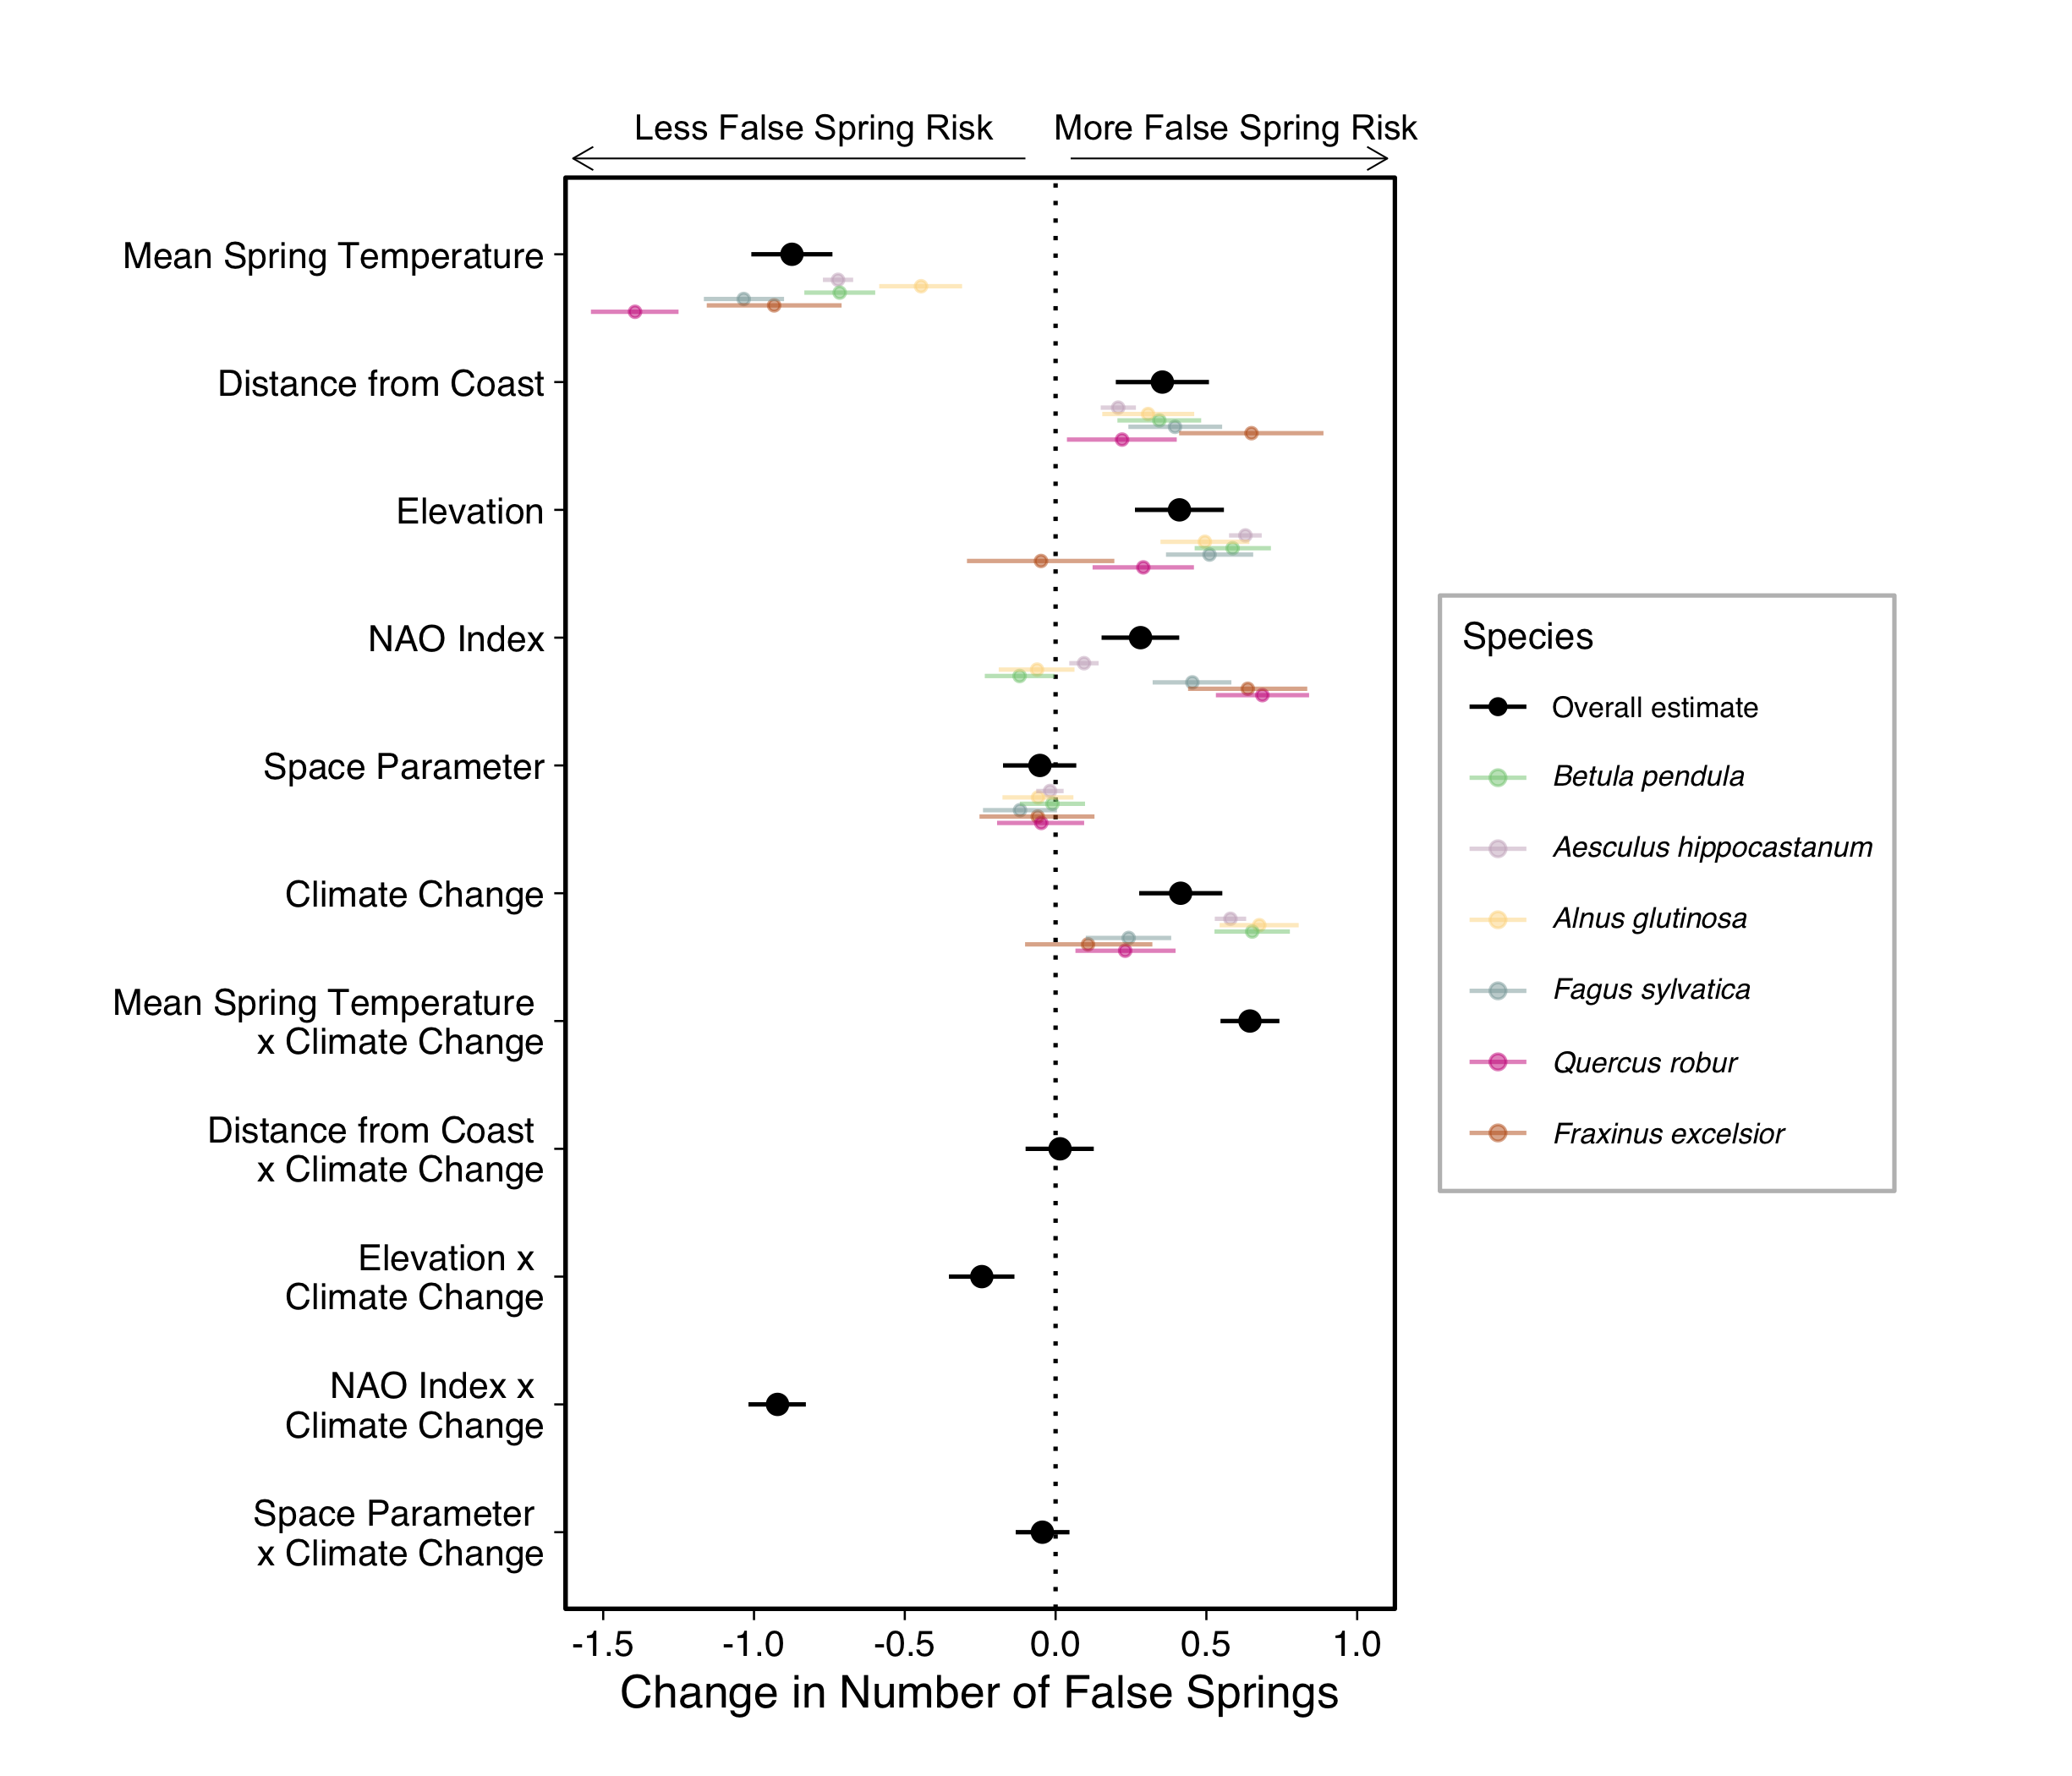
\includegraphics[width=12cm]{..//analyses/figures/model_output_90_fivespp.png}
  -\caption{Effects of species, climatic and geographical predictors on false spring risk with a lower temperature threshold (-5$^{\circ}$C) for defining a false spring. More positive values indicate an increased probability of a false spring whereas more negative values suggest a lower probability of a false spring. Dots and lines show means and 90\% uncertainty intervals. Values closer to zero have less of an effect on false springs. There were 730,996 zeros and 23,855 ones for false springs in the data.}\label{fig:five}
  -\end{center}
  -\end{figure}}
  
% latex table generated in R 3.6.0 by xtable 1.8-4 package
% Fri Oct  4 09:51:54 2019
\begin{longtable}{lrrrrr}
\caption{Summary of Bernouilli model of false spring risk with a lower temperature threshold (-5$^{\circ}$C) for defining a false spring without the species interactions (estimates presented on logit scale for \textit{Aesculus hippocastanum}).} \\ 
  \hline
 & Estimate & 10\% & 25\% & 75\% & 90\% \\ 
  \hline \endhead  \hline
Intercept & -3.35 & -3.37 & -3.36 & -3.34 & -3.32 \\ 
  NAO Index & 0.09 & 0.05 & 0.07 & 0.11 & 0.14 \\ 
  Mean Spring 
Temperature & -0.72 & -0.77 & -0.74 & -0.70 & -0.67 \\ 
  Distance from 
Coast & 0.21 & 0.15 & 0.18 & 0.23 & 0.27 \\ 
  Elevation & 0.63 & 0.58 & 0.61 & 0.65 & 0.68 \\ 
  Space Parameter & -0.02 & -0.06 & -0.04 & 0.00 & 0.03 \\ 
  Climate Change & 0.58 & 0.53 & 0.56 & 0.60 & 0.63 \\ 
  Alnus glutinosa & 0.33 & 0.28 & 0.31 & 0.34 & 0.37 \\ 
  Betula pendula & 0.08 & 0.04 & 0.06 & 0.09 & 0.12 \\ 
  Fagus sylvatica & -0.45 & -0.49 & -0.46 & -0.43 & -0.40 \\ 
  Fraxinus excelsior & -1.58 & -1.66 & -1.61 & -1.55 & -1.50 \\ 
  Quercus robur & -1.26 & -1.32 & -1.28 & -1.24 & -1.20 \\ 
  NAO Index
by Alnus glutinosa & -0.16 & -0.23 & -0.19 & -0.12 & -0.08 \\ 
  NAO Index
by Betula pendula & -0.21 & -0.28 & -0.24 & -0.19 & -0.15 \\ 
  NAO Index
by Fagus sylvatica & 0.36 & 0.28 & 0.33 & 0.39 & 0.44 \\ 
  NAO Index
by Fraxinus excelsior & 0.54 & 0.39 & 0.48 & 0.60 & 0.69 \\ 
  NAO Index
by Quercus robur & 0.59 & 0.49 & 0.55 & 0.63 & 0.70 \\ 
  Mean Spring 
Temperature
by Alnus glutinosa & 0.28 & 0.19 & 0.24 & 0.31 & 0.36 \\ 
  Mean Spring 
Temperature
by Betula pendula & 0.01 & -0.06 & -0.02 & 0.03 & 0.07 \\ 
  Mean Spring 
Temperature
by Fagus sylvatica & -0.31 & -0.39 & -0.35 & -0.28 & -0.23 \\ 
  Mean Spring 
Temperature
by Fraxinus excelsior & -0.21 & -0.39 & -0.28 & -0.14 & -0.04 \\ 
  Mean Spring 
Temperature
by Quercus robur & -0.67 & -0.77 & -0.71 & -0.63 & -0.58 \\ 
  Distance from 
Coast
by Alnus glutinosa & 0.10 & 0.01 & 0.06 & 0.14 & 0.19 \\ 
  Distance from 
Coast
by Betula pendula & 0.14 & 0.06 & 0.10 & 0.17 & 0.22 \\ 
  Distance from 
Coast
by Fagus sylvatica & 0.19 & 0.09 & 0.15 & 0.23 & 0.29 \\ 
  Distance from 
Coast
by Fraxinus excelsior & 0.44 & 0.26 & 0.37 & 0.52 & 0.62 \\ 
  Distance from 
Coast
by Quercus robur & 0.01 & -0.11 & -0.04 & 0.06 & 0.14 \\ 
  Elevation
by Alnus glutinosa & -0.13 & -0.23 & -0.17 & -0.10 & -0.04 \\ 
  Elevation
by Betula pendula & -0.04 & -0.11 & -0.07 & -0.01 & 0.03 \\ 
  Elevation
by Fagus sylvatica & -0.12 & -0.21 & -0.16 & -0.08 & -0.03 \\ 
  Elevation
by Fraxinus excelsior & -0.68 & -0.87 & -0.75 & -0.60 & -0.49 \\ 
  Elevation
by Quercus robur & -0.34 & -0.45 & -0.39 & -0.29 & -0.22 \\ 
  Space Parameter
by Alnus glutinosa & -0.04 & -0.11 & -0.07 & -0.01 & 0.03 \\ 
  Space Parameter
by Betula pendula & 0.01 & -0.05 & -0.02 & 0.03 & 0.07 \\ 
  Space Parameter
by Fagus sylvatica & -0.10 & -0.18 & -0.13 & -0.07 & -0.02 \\ 
  Space Parameter
by Fraxinus excelsior & -0.04 & -0.19 & -0.10 & 0.02 & 0.10 \\ 
  Space Parameter
by Quercus robur & -0.03 & -0.13 & -0.07 & 0.01 & 0.07 \\ 
  Climate Change
by Alnus glutinosa & 0.10 & 0.02 & 0.06 & 0.13 & 0.17 \\ 
  Climate Change
by Betula pendula & 0.07 & -0.00 & 0.04 & 0.10 & 0.14 \\ 
  Climate Change
by Fagus sylvatica & -0.34 & -0.43 & -0.37 & -0.30 & -0.25 \\ 
  Climate Change
by Fraxinus excelsior & -0.47 & -0.63 & -0.54 & -0.41 & -0.31 \\ 
  Climate Change
by Quercus robur & -0.35 & -0.46 & -0.40 & -0.30 & -0.23 \\ 
  NAO Index by Climate Change & -0.92 & -1.02 & -0.96 & -0.88 & -0.83 \\ 
  Mean Spring 
Temperature by Climate Change & 0.64 & 0.55 & 0.60 & 0.69 & 0.74 \\ 
  Distance from 
Coast by Climate Change & 0.01 & -0.10 & -0.03 & 0.06 & 0.13 \\ 
  Elevation by Climate Change & -0.24 & -0.35 & -0.29 & -0.20 & -0.14 \\ 
  Space Parameter by Climate Change & -0.04 & -0.13 & -0.08 & -0.01 & 0.05 \\ 
   \hline
\hline
\end{longtable}


\end{document}
